\documentclass{article}
\usepackage[utf8]{inputenc}
\usepackage{hyperref}

\title{Übung 4}
\author{Laurenz Weixlbaumer, 11804751}
\date{November 2018}

\renewcommand\thesubsection{(\alph{subsection})}

\usepackage{enumitem}
\usepackage{mathtools}

\begin{document}

\maketitle

\stepcounter{section}\stepcounter{section}\stepcounter{section}
\section{Komparatoren}

Der \emph{Add/Sub} Block stellt das Additions-Subtraktionswerk aus \textbf{2.} dar.

\begin{enumerate}[label=(\alph*)]

\item Kleiner Operator ($K1 = A < B$)

\begin{figure}[htp]
\begin{center}
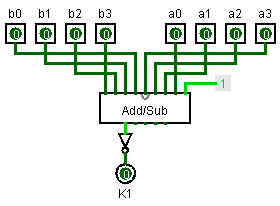
\includegraphics[width=6cm]{comp_sm_circuit.png}
\end{center}
\end{figure}

\item Größer Gleich Operator ($K2 = A \geq B$)

\begin{figure}[htp]
\begin{center}
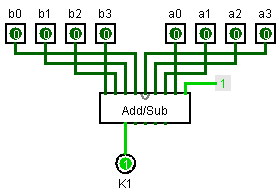
\includegraphics[width=6cm]{comp_grq_circuit.png}
\end{center}
\end{figure}

\end{enumerate}

\end{document}
